\documentclass[a4paper, fleqn]{article}
\usepackage[utf8]{inputenc}
\usepackage{amsmath}
\usepackage{amssymb}
\usepackage{caption}
\usepackage{mathtools}
\usepackage{amsfonts}
\usepackage{lastpage}
\usepackage{tikz}
\usepackage{float}
\usepackage{textcomp}
\usetikzlibrary{patterns}
\usepackage{pdfpages}
\usepackage{gauss}
\usepackage{fancyvrb}
\usepackage[table]{colortbl}
\usepackage{fancyhdr}
\usepackage{graphicx}
\usepackage{hyperref}
\usepackage[margin=2.5 cm]{geometry}

\setlength\parindent{0pt}
\setlength\mathindent{75pt}

\definecolor{listinggray}{gray}{0.9}
\usepackage{listings}
\lstset{
	language=,
	literate=
		{æ}{{\ae}}1
		{ø}{{\o}}1
		{å}{{\aa}}1
		{Æ}{{\AE}}1
		{Ø}{{\O}}1
		{Å}{{\AA}}1,
	backgroundcolor=\color{listinggray},
	tabsize=3,
	rulecolor=,
	basicstyle=\scriptsize,
	upquote=true,
	aboveskip={0.2\baselineskip},
	columns=fixed,
	showstringspaces=false,
	extendedchars=true,
	breaklines=true,
	prebreak =\raisebox{0ex}[0ex][0ex]{\ensuremath{\hookleftarrow}},
	frame=single,
	showtabs=false,
	showspaces=false,
	showlines=true,
	showstringspaces=false,
	identifierstyle=\ttfamily,
	keywordstyle=\color[rgb]{0,0,1},
	commentstyle=\color[rgb]{0.133,0.545,0.133},
	stringstyle=\color[rgb]{0.627,0.126,0.941},
  moredelim=**[is][\color{blue}]{@}{@},
}

\lstdefinestyle{base}{
  emptylines=1,
  breaklines=true,
  basicstyle=\ttfamily\color{black},
}

\def\checkmark{\tikz\fill[scale=0.4](0,.35) -- (.25,0) -- (1,.7) -- (.25,.15) -- cycle;}
\newcommand*\circled[1]{\tikz[baseline=(char.base)]{
            \node[shape=circle,draw,inner sep=2pt] (char) {#1};}}
\newcommand*\squared[1]{%
  \tikz[baseline=(R.base)]\node[draw,rectangle,inner sep=0.5pt](R) {#1};\!}
\newcommand{\comment}[1]{%
  \text{\phantom{(#1)}} \tag{#1}}
\def\A{\mathcal{A}}
\def\I{\mathcal{I}}
\def\E{\mathbb{E}}
\def\el{[\![}
\def\er{]\!]}
\def\dpip{|\!|}
\def\MeanN{\frac{1}{N}\sum^N_{n=1}}
\cfoot{Page \thepage\ of \pageref{LastPage}}
\DeclareGraphicsExtensions{.pdf,.png,.jpg}
\begin{document}
\section*{Reading}
\begin{itemize}
    \item RA 2
    \item \url{https://en.wikipedia.org/wiki/Yao\%27s\_principle}
\end{itemize}
\tableofcontents
\section{Game Tree}
% MIN = even = AND
% MAX = odd  = OR
\subsection{Definintion}
We let $T_{d,k}$ be a tree of height $2k$ where at each node there are $d$ children. Lets discuss trees with $d=2$, eg. binary trees, where every node is a OR node if has odd length to the root, every other node is an AND node. Each leaf is either 0 or 1. Our game tree evaluates either to 1 or to 0. We want to study the maximum number of steps it takes to evaluate any instance of $T_{2,k}$.\\
For any deterministic algorithm, it is easy to see that we can always formulate leaves such that all must be checked. Thus our worst case number of steps is $2^{2k} = 4^k$.\\
We propose a simple randomized algorithm, where evaluation of children at a node is chosen at random, resulting at an expected cost of evaluation of any instance of $T_{2,k}$ is at most $3^k$.
\subsection{Proof}
We will prove the above by induction.
\subsubsection*{Base: $k=1$}
We have a tree
\begin{verbatim}
           AND
          /   \
        OR     OR
       /  \   /  \
      ?    ? ?    ?
\end{verbatim}
Our OR nodes need to evaluate both children if they are 0, and only one if they are both 1, and expected 3/4 if they are mixed.
Our AND need to evaluate both children if they are 1, only one if they are both 0, and expected 3/4 if they are mixed.
Meaning we have an expected number of leaves inspected being:
$$
 (1/4 * 2 + 1/4 + 1/4 + 1/4 * 2)^2 = (3/2)^2 = 9/4 < 3^1
$$
\subsubsection*{Step}
We assume the expected cost of evaluating any instance of $T_{2,k-1}$ is $3^{k-1}$.\\
We consider a tree $T$ with an OR root node, if it were to evaluate to 1, at least one of its children returns 1. We pick this child with probability a half, giving us an expected cost of at most $3^{k-1}$ in evalutation $T$. With probability at most $1/2$ both subtrees are evaluated, giving us a cost of at most $2 * 3^{k-1}$. In this case our expected cost is
$$
1/2 * 3^{k-1} + 1/2 * 2 * 3^{k-1} = 3/2 * 3^{k-1}
$$
In the case where $T$ evaluates to 0, both children must be evaluated, giving us a cost of $2 * 3^{k-1}$.
If we consider the root of the tree $T$ being an AND node. If it evaluates to 1, both subtrees must return 1. By the above argument and by linearity of expectation, the expected cost of evaluating $T$ to 1 is at most $2 * 3/2 * 3^{k-1} = 3^k$. In the case that $T$ evaulates to 0, at least one of its children evaluate to 0, this child is chosen first with probability 1/2, so the expected cost of evaluating $T$ is at most
$$
2*3^{k-1} + 1/2 * 3/2 * 3^{k-1} = 11/4 * 3^{k-1} \leq 3^k
$$
since $n= 4^k$ the expected running time of our randomized algorithm is at most $n^{\log_4 3} \leq n^{0.793}$
\section{Yao's minimax}
\subsection{Definition}
For all distributions $p$ over $\I$ and $q$ over $\A$, where C(I,A) is the cost of running algorithm A on input I.
$$
\min_{A \in \A} \E[C(I_p, A)] \leq \max_{I\in\I} \E[C(I,A_q)]
$$
ie. the expected running time of the optimal deterministic algorithmen for an arbitrarily chosin input distribution $p$ ias a lower bound on the expected running time of the optimal Las Vegas randomized algorithm for the problem.
\subsection{Proof}
We define $q \in Q$ as all the input probabilities, and $p\in P$ as all the algorithm probability distributions, $A_q$ is the algorithm chosen according to the probability distribution $q$ and $I_p$ as the input according to the probability distribution $p$.\\
We let $c = \max_{I\in\I} \E[C(I,A_q)]$. For every input $I$, we have $\sum_{q \in Q} q C(I,A_q) \leq c$. Therefore we have
$$\sum_{p \in P} p \sum_{q \in Q} q C(I_p,A_q) \leq c.$$
As all terms are non-negative we can switch order of summation giving us
$$\sum_{q \in Q} q \sum_{p \in P} p C(I_p,A_q) \leq c.$$
By the Pigeonhole principle there must exist an algorithm $A_q$ such that $\sum_{p \in P} p C(I_p,A_q) \leq c$, concluding the proof.
\section{Yao on Game Tree}
A tree $T_{2,k}$ is equivalent to a balanced binary tree of whose leaves are at distance 2k from the root, where nodes compute the NOR function.
We want to analyse this tree of NORs with depth 2k using Yao's Minimax principle to prove a lower boundon the expected number of leaves evaluated by any randomized algorithm.
We here chose the input probability, i.e. the probability that a leaf is 1, to be $p = (3 - \sqrt{5})/2$. We note that if each input to a NOR node is independently 1 iwht probability p, then the probability that its output is 1 is the probability that both its inputs are 0, which is:
$$
(1 - p)^2 = \left(\frac{\sqrt 5 - 1}{2} \right)^2 = \frac{3-\sqrt{5}}{2} = p
$$
\paragraph{Prop 2.7 (USED WITHOUT PROOF)} Let $T$ be a NOR tree each of whose leaves is independently set to 1 with probability q for a fixed value $q \in [0,1]$. Let $W(T)$ denote the minimum over all deterministic algorithms, of the expected number of steps to evaluate $T$. Then there is a depth-first pruning algorithm whose expected number of steps to evaluate $T$ is $W(T)$\\
For a depth first pruning algorithm evaluating this tree, we let $W(h)$ be the expected number of leaves it inspects in determining the value of a node at distance $h$ from the leaves, then
$$
W(h) = W(h-1) + (1-p) * W(h-1)
$$
If we let $h$ be $\log_2(n)$ and solve we get $W(h) \geq n^{0.694}$
\newpage
\begin{center}
  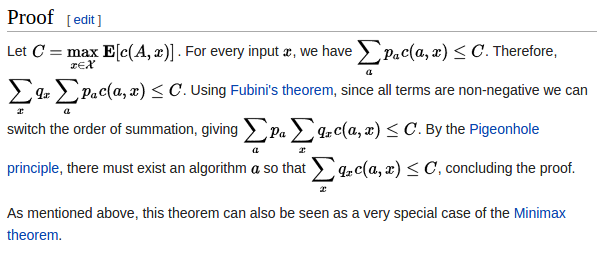
\includegraphics[scale=0.7]{./notes_2_gametheory_yao.png}
\end{center}
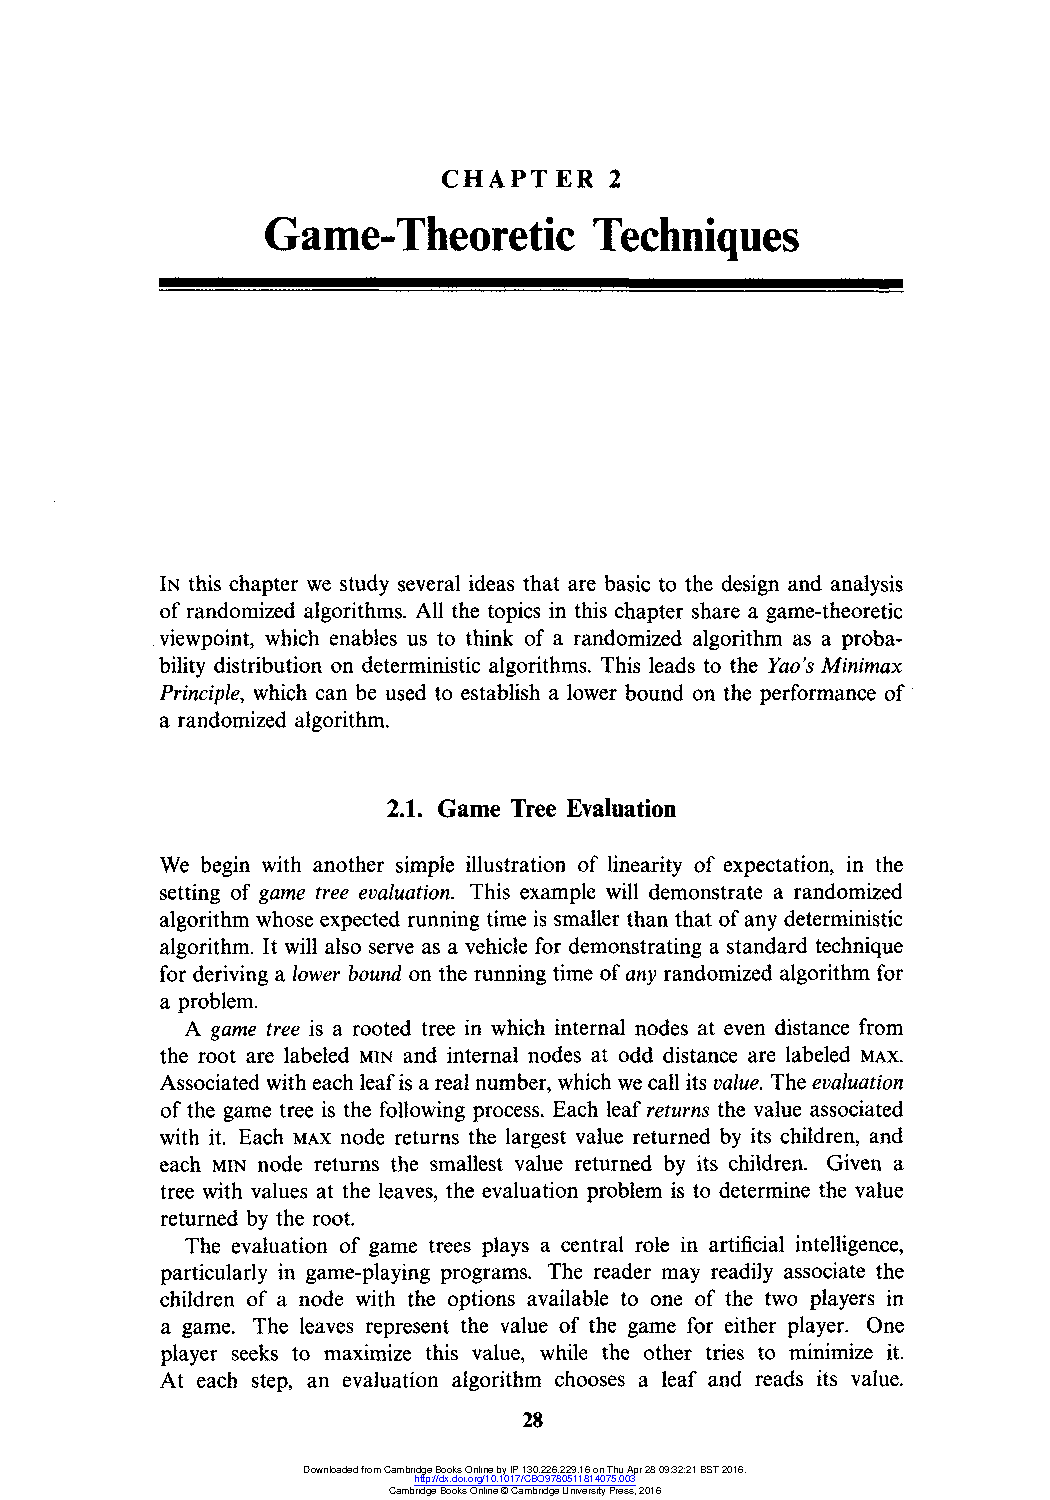
\includepdf[pages=-]{./notes_2_gametheory.pdf}
\end{document}
